\chapter{Technologies Employed}
\label{ch:techs}

In this Chapter, we will go over the different technologies that compose the system built for SpazioDati, as it was outlined in Figure \ref{fig:cdc-complete}.


\section{Apache Kafka}
\label{sec:kafka}

Before stating what Apache Kafka is, the reader will find it clearer if we introduce the log data structure first.
That is, an unbounded, append-only sequence of records,\footnote{%
	Or messages, or events, etc.
} ordered by time.
For the purposes of a log sequence, let us disregard a precise notion of time; instead, let us loosely assert that subsequent messages were recorded (and received) subsequently.

Kafka, at its core, is a distributed system which handles logs, whilst providing desirable features for such systems: fault-tolerance, high throughput, low latency, and responsiveness to unwanted network partitioning.

Kafka itself is a cluster of independent broker systems, which operate together making use of the Paxos\footnote{%
	Cf. \cite{paxos}.
} protocol to provide Kafka's functionalities.

Architecturally, as outlined in Figure \ref{fig:kafka-architecture}, the overall system entails the presence of some Producers (which send records to the cluster), and Consumers (which read records from the cluster).
These two sets of systems, which do not strictly pertain to Kafka but base their operations on its features, are completely decoupled from one another, even if, generally it is by the combination of them that a particular purpose is achieved.
This is a desirable characteristic of the overall system, which enables interoperability between even vastly heterogeneous producer and consumer systems.

\begin{figure}
	\centering
	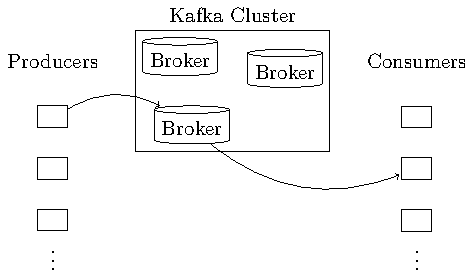
\includegraphics[height=5cm]{figures/technologies/kafka-architecture}
	\caption{General overview of Kafka Architecture.}
	\label{fig:kafka-architecture}
\end{figure}

In Kafka's terminology, which is common in the field, records belong to topics; i.e. named logs.
A Producer will instruct Kafka to store a record and that it pertains to a particular topic.
Conversely, a Consumer will ask Kafka to read a record from a particular topic, at some specific offset.

A topic is further divided into so called partitions.\footnote{%
	Therefore, to be precise, each single topic partition is a log and a topic is a set of logs.
	Nonetheless, in our use-case, as discussed shortly, we will not split topics into multiple partitions, thus leaving little space to imprecision.
}
Generally, this division is most useful when considering the capability of some greater system, which is in part composed by Kafka, to meet increasing computational demands.
This is achieved by dividing homogeneous records into different partitions that are read by separate Consumers, thus enabling greater simplicity in the addition of Consumers, therefore expanding the computing capability assigned to the consumption of records.

Since each partition is a log in itself, records are inherently ordered, but ordering \emph{between} partitions is not guaranteed, unless records are assigned to some key, which in our use case coincides with the primary key.
If this assignment is made, then records pertaining to a particular key will always be assigned to the same partition; hence, the necessary ordering of streamed records is preserved (cf. \S \ref{sec:tables-streams}).
Meeting greater computational demands can therefore be achieved through this mean.
Nevertheless, the presented implementation does not make use of this mechanism, because of development time limitations.

In our use case each table that is being reproduced from the data source, will be assigned to a different topic.
Each table-topic will be read from separate Consumers, as better explained in the following \S \ref{sec:kafka-connect}.

One interesting aspect of Kafka's design is the pervasive and efficient usage of persistent memory, described in detail in \cite[\S 4.2, and \S 4.3]{kafka-docs}.
Seeing how disk read operations can have a throughput similar to that of a computer network,\footnote{%
	Cf. \cite{pathologies-big-data}.
} the following statement from Kafka's Documentation makes a lot of sense:
\begin{quote}
	[\ldots] Rather than maintain as much as possible in-memory and flush it all out to the filesystem in a panic when we run out of space, we invert that. All data is immediately written to a persistent log on the filesystem without necessarily flushing to disk. In effect this just means that it is transferred into the kernel's pagecache.
\end{quote}

Thus, instead of spawning a memory management subsystem for its own purposes, Kafka relinquishes control and relies on the OS to handle its persistent memory.
Kafka also uses the \cite[\texttt{sendfile}(2)]{linux-man} system call for greater efficiency in I/O operations when receiving from or sending records over the network.
A \texttt{sendfile} call directs data from an input file descriptor to an output file descriptor, without leaving the kernel-space, thus saving the programmer from having an additional buffer in user-space.


\subsection{Kafka Connect}
\label{sec:kafka-connect}

From Kafka's documentation:
\begin{quote}
	Kafka Connect is a tool for scalably and reliably streaming data between Apache Kafka and other systems. It makes it simple to quickly define connectors that move large collections of data into and out of Kafka.\footcite[\S 8.1]{kafka-docs}
\end{quote}

\sloppy Kafka Connect provides two abstractions over very common use-cases, namely Source and Sink Connectors.
Effectively, with regards to the terminology previously introduced, a Source Connector is a Producer and a Sink Connector is a Consumer.
The switch in terminology is due to the fact that any Connector is entirely managed by the Kafka Connect runtime, implying that some of their logic is managed by Connect.
Thus, developers are inevitably more restricted in their design choices over Connectors; nonetheless, this restriction provides greater simplicity in the definition of Producers and Consumers that follow the common pattern stated in the above quotation, which is the rationale for Kafka Connect itself.

\fussy In order to allow external control, Kafka Connect provides a REST interface utilized for starting, stopping, pausing, and resuming Connectors, along with more functionalities designed to manage Kafka Connect itself.
The rest of the operations are all managed internally, without the need for manual control.

In our case, we will have Debezium Source Connectors (cf. \S \ref{sec:debezium}) for each source database, and as many Sink Connectors as there are tables in the output database.
The code Sink Connectors use was purpose-built and can be found in Listing \ref{src:eu.spaziodati.metrics/connectors/PostgresSinkTask.scala}, which will be explained in greater detail in the following chapters.
For the purposes of this Section, it will suffice to say that the listed code generates a Sink Connector Task, which is responsible for handling the transfer of data out of Kafka and into the output database.


\subsection{Kafka Streams}
\label{sec:kafka-streams}

Kafka Streams is a library that conveys various utilities for developing systems that operate with Kafka, most importantly it addresses systems that act both as consumers and as producers at the same time.
In particular, this underlies the concept of a stream, intended as the computation carried out by a chain of Producers that write to certain topics, Consumers that read from said topics as well as produce to other topics, and so forth.

Recalling our previous assertions on the duality of streams and tables (cf. \S \ref{sec:tables-streams}), let us utilize such a notion to state the usage of Kafka Streams in our application.
Since a stream can be interpreted as a table, modifications coherently applied to all records of a stream constitute changes to a table, thus the operations of relational algebra can be adapted and applied to streams as well.
I will not endeavor into a formal demonstration of this notion, nonetheless I will try to convince the reader that this is true in the code provided.

In our case, Kafka Streams are employed for the aggregations regarding certain tables, that will be described in \S \ref{sec:aggregations}.
The code for components of the proposed system that make use of Kafka Streams are presented in Listings \ref{src:eu.spaziodati.metrics/streams/etaStream.scala}, \ref{src:eu.spaziodati.metrics/streams/kappaStream.scala},
\ref{src:eu.spaziodati.metrics/streams/lambdaStream.scala}, and
\ref{src:eu.spaziodati.metrics/streams/thetaStream.scala}.

For instance, let us consider table $\eta$. In Query (\ref{agg:eta}), defined in the next Chapter, we have a grouping\footnote{%
	Recall Definition \ref{def:G}.
} with keys user, time, and class. In Listing \ref{src:eu.spaziodati.metrics/streams/etaStream.scala}, lines 29 -- 39, we utilize the Kafka Streams APIs to achieve the operation $G_{\text{user, time, class}}(\source{\eta})$.
The subsequent grouping selection\footnote{%
	Recall Definition \ref{def:sigma*}.
} is performed on lines 48 and 49.

By looking at this example, the difference with the notation proposed in Chapter \ref{ch:intro} is evident.
While the operator $\sigma^*$ points to the result of the aggregation, for instance in this case $\sum$, on line 49 we compute the value one data change event at a time.
This difference is in line with the duality expressed in \S \ref{sec:tables-streams}.


\section{PostgreSQL}

While a detailed discussion of the several technologies involved in operating the presented system is the intent of this Chapter, because of the fact that the great majority of the intended audience for this document already has knowledge on this topic and that the discussion itself would be too broad, an explanation of what a relational database is, is intentionally left to the several books\footnote{%
	E.g. \cite{dbms}, \cite{db-systems}.
} that already provide a thorough discussion.

Nonetheless, in this Section, particular aspects of the PostgreSQL relational database will be presented, when they directly pertain contents of this Thesis.


\subsection{Write Ahead Log}
\label{sec:wal}

The Write Ahead Log (WAL) is a core component of PostgreSQL servers, and similar implementations are present in most relational databases.
Its function is to log transactional data, i.e. data referred to some transaction, as defined in \cite[\S 16.2]{dbms}.

Such a log provides data integrity.
Power loss, OS failure, or hardware failure\footnote{%
	Except when related to the persistent storage itself.
	Evidently, should such be the nature of hardware failure, no action can provide data integrity.
} can impede successful flushing of all data pages to disk, but writing the transactional changes themselves on a log, an operation far less costly due to the inherent sequential writing, is sufficient to later recover the data to a consistent state.
As the name suggests, data is logged in the WAL before it is written to persistent storage, which is the reason why integrity is preserved.

Some further remarks in PostgreSQL's Documentation:
\begin{quote}
	Using WAL results in a significantly reduced number of disk writes, because only the log file needs to be flushed to disk to guarantee that a transaction is committed, rather than every data file changed by the transaction. The log file is written sequentially, and so the cost of syncing the log is much less than the cost of flushing the data pages. This is especially true for servers handling many small transactions touching different parts of the data store. Furthermore, when the server is processing many small concurrent transactions, one fsync of the log file may suffice to commit many transactions.\footnote{%
		From \cite[\S 29.2]{pg-docs}
	}
\end{quote}

For a more detailed explanation, refer to \cite[Chapter 29]{pg-docs}.


\subsection{Logical Replication}
\label{sec:pg-replication}

In addition to what's already been stated, the aforementioned WAL is used by PostgreSQL in order to provide the feature of logical replication.
It is a process by which external systems can consume data from the WAL, thus essentially replicating the database contents.

Data is extracted and logically decoded;\footnote{
	I.e. transformed in a format that is suited to be understood by systems other than PostgreSQL; see \cite[Chapter 48]{pg-docs} for details.
} next it is exported through a replication slot, which essentially transmits the data to some external system that can then use it according to its needs.


\section{Debezium}
\label{sec:debezium}

Debezium is a Source Connector (cf. \ref{sec:kafka-connect}), developed by Red Hat.\footnote{%
	See \cite{debezium-docs}.
}
It possesses the capability of extracting data change events from various relational database management systems, including PostgreSQL.
Then, regardless of the kind of data source, it writes data to Kafka topics.

In particular, when extracting data from a PostgreSQL server, Debezium utilizes the means described in the previous Sections \ref{sec:wal}, and \ref{sec:pg-replication}.

In our case, Debezium is configured to listen (by means of replication slots) to changes on tables from the source databases; specifically there is one Debezium Connector for each source database.\footnote{%
	In fact, a single Debezium Connector cannot simultaneously connect to multiple databases.
}
Then, data regarding each individual table is sent to a specific topic, as already stated in \S \ref{sec:kafka}.

As will be stated in later chapters,\footnote{%
	See \ref{sec:foreign-key}.
} the independence of parallel processing between separate table-topics is an important aspect of the presented system's implementation.


\section{Scala}

Scala is the programming language of choice for a substantial part of work done for the proposed system's implementation.
The selection of source code displayed in Appendix \ref{ch:source} is entirely written in Scala.

The following are some of Scala's features, as noted from its authors:
\begin{quote}
	\begin{itemize}
		\item It’s a high-level language;
		\item It’s statically typed;
		\item Its syntax is concise but still readable -- we call it \emph{expressive};
		\item It supports the object-oriented programming (OOP) paradigm;
		\item It supports the functional programming (FP) paradigm;
		\item It has a sophisticated type inference system;
		\item Scala code results in .class files that run on the Java Virtual Machine (JVM);
		\item It’s easy to use Java libraries in Scala.\footnote{%
			From \cite[Prelude: A Taste of Scala]{scala-book}.
		}
	\end{itemize}
\end{quote}

Personally, I have learned Scala whilst fulfilling the curricular internship mentioned in Chapter \ref{ch:intro}; a learning process which I remarkably enjoyed.

